\documentclass{article}
\usepackage{gensymb, amsmath, float, graphicx}
\restylefloat{table}
\usepackage[margin=0.75in]{geometry}
\usepackage{verbatim}
\begin{document}

\title{Ocean Bowl Bootcamp 3: Plate Tectonics}
\author{Michael Shen}
\maketitle

\section{Quick Summary}

\begin{itemize}
	\item The theory of plate tectonics was developed to explain phenomena such as continental drift (Alfred \textbf{Wegener}). While there are a lot of tectonic plates, the main ones (the ones everyone should remember) are attached at the end (Figure 1).
	
	\item Plate tectonics states that the solid \textbf{lithosphere} of the Earth drifts on top of a liquid \textbf{asthenosphere}. Note that the lithosphere contains the crust and the upper, still solid, regions of the mantle. The asthenosphere is completely liquid.
	
	\item There are two types of plates, \textbf{continental} and \textbf{oceanic}. They have different compositions and thus behave slightly differently; oceanic plates are \textbf{mafic}, that is, containing high Mg and Fe content, while continental plates are \textbf{felsic}, that is, containing high feldspar and silica content. 
	
	
	\begin{itemize}
		\item The most common mafic rock is \textbf{basalt}, while the most common felsic rock is \textbf{granite}.
		\item The terms also extend to volcanic activity. Those who have taken Chemistry AP can search for and understand the chemical reasons, but the higher the $SiO_2$ content, the more viscous the magma. This means that \textbf{felsic magma} is more viscous and results in more explosive eruptions (think Mt. St. Helens). \textbf{Mafic magma} is, on the other hand, less viscous and tends to result in free-flowing eruptions (think Mauna Loa).
	\end{itemize}
	
	
	\begin{table}[h]
	\centering
		\begin{tabular}{c|c|c}
		\textbf{SiO2 Content} & \textbf{Magma Type} & \textbf{Volcanic Rock} \\ \hline
		~50\% & Mafic & Basalt \\
		~60\% & Intermediate & Andesite \\
		~65\% & Felsic & Dacite \\
		~70\% & Felsic & Rhyolite
		\end{tabular}
		\caption{Types of igneous rock formed based on $SiO_2$ content in the magma}
	\end{table}
	
	\item \textbf{Hotspots} are areas where the magma from the mantle rises up and through the lithosphere away from any plate boundary. Since they originate from the mantle, they are stationary relative to the motion of the lithosphere above it, that is, hot spots remain at approximately the same location while tectonic plates move past them (Figure 2). Good examples include the Hawaii/Emperor Seamount Islands and Yellowstone.

	\item There are three main types of plate boundaries: \textbf{divergent}, \textbf{convergent}, and \textbf{transform} (Figures 3, 4).
	
	
	\begin{itemize}
		\item A continental-continental convergence forms a mountain range via \textbf{uplifting} - no volcanic activity is created. Oceanic-oceanic convergence and oceanic-continental convergence behave similarly, with a \textbf{subduction} zone forming a trench and generating volcanic activity.
		\item The divergent boundary to know is the \textbf{Mid-Atlantic Ridge}. Located on the divergent boundary in the middle of the Atlantic Ocean, it is technically the longest mountain chain in the world and has enabled many useful discoveries, such as the ability to historically map the Earth's magnetic field over time.
	\end{itemize}
	

\end{itemize}

\section{Figures}
\begin{figure}[H]
	\centering
	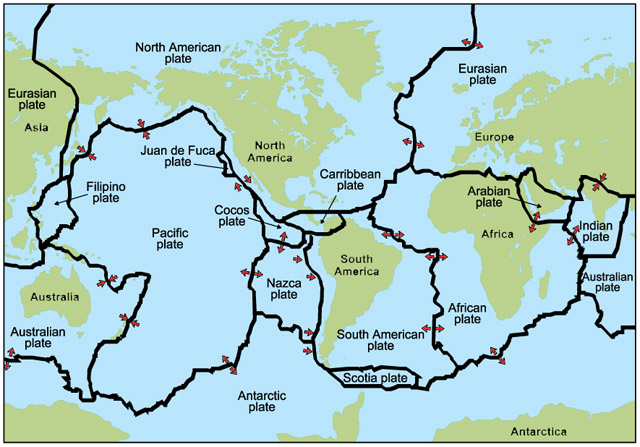
\includegraphics[width=\textwidth]{./Images/BC3_PlateMap.jpg}
	\caption{Map of the major tectonic plates; memorize the names of the plates!}
\end{figure}
\begin{figure}[H]
    \centering
    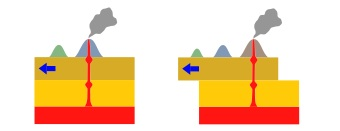
\includegraphics{./Images/BC3_Hotspot.jpg}
    \caption{Simple diagram illustrating the behavior of a geological hotspot}
\end{figure}
\begin{figure}[H]
    \centering
    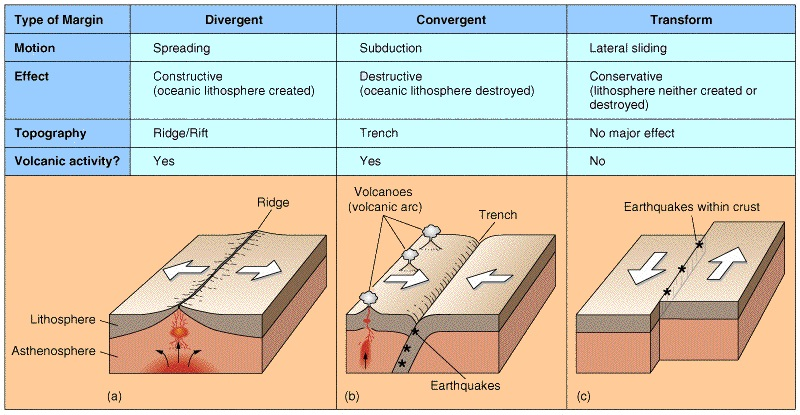
\includegraphics[width=\textwidth]{./Images/BC3_PlateBoundary.jpg}
    \caption{Diagram of typical plate boundary behavior, with oceanic-continental convergence}
\end{figure}
\begin{figure}[H]
    \centering
    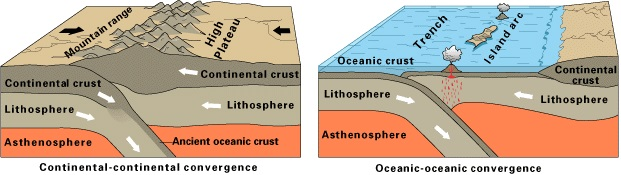
\includegraphics{./Images/BC3_PlateBoundaryC.jpg}
    \caption{Diagram of typical continental-continental and oceanic-oceanic plate convergence behavior}
\end{figure}

\end{document}